\newpage

\section{ARP Poisoning}
\subsection{Activity}

\noindent {\bf{Bước 1:}} Khởi động Kali Linux VM từ phần 2. Vào \textbf{Terminal}, nhập lệnh \textbf{ifconfig}.

\begin{figure}[!htb]
    \centering
    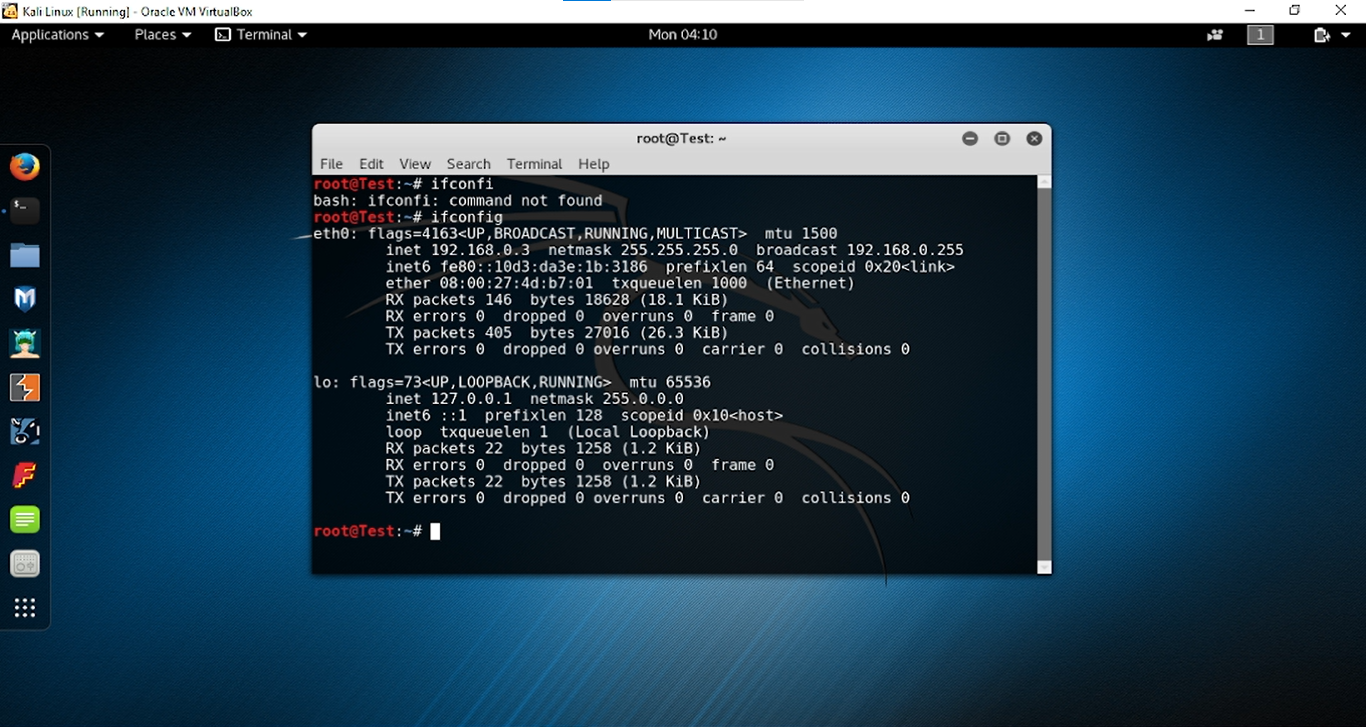
\includegraphics[width=1\linewidth]{figure//chapter5//lab5_3/if-config_ver2.png}
    \caption{Kết quả khi chạy ifconfig trên Kali Linux 2016 VM}
    \label{fig:enter-label}
\end{figure}

\noindent {\bf{Bước 2:}} Ở Windows Server và Windows 10, thực hiện lệnh \textbf{ipconfig /all} ở \textbf{cmd} và lưu lại địa chỉ IP.

\begin{figure}[!htb]
    \centering
    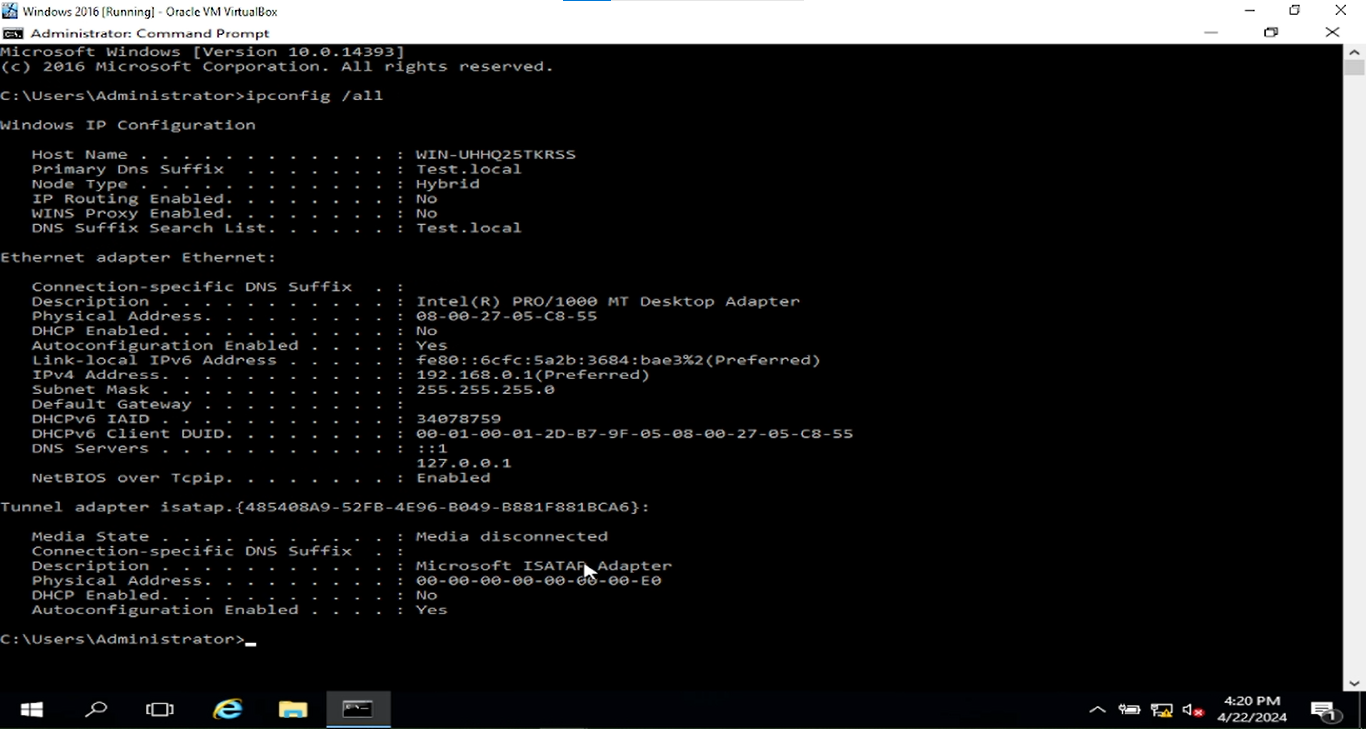
\includegraphics[width=1\linewidth]{figure//chapter5//lab5_3/ipconfig_windows.png}
    \caption{Kết quả khi chạy ipconfig trên Windows 10}
    \label{fig:enter-label}
\end{figure}

\newpage

\noindent {\bf{Bước 3:}} Thực hiện \textbf{ping 192.168.0.2} từ Windows Server tới Windows 10. Kết quả chưa nhận được request, tuy nhiên hai máy này đã có thể nhận được giá trị địa chỉ IP và địa chỉ MAC của nhau. Kết quả có thể thấy được từ lệnh \textbf{arp -a}.

\begin{figure}[!htb]
    \centering
    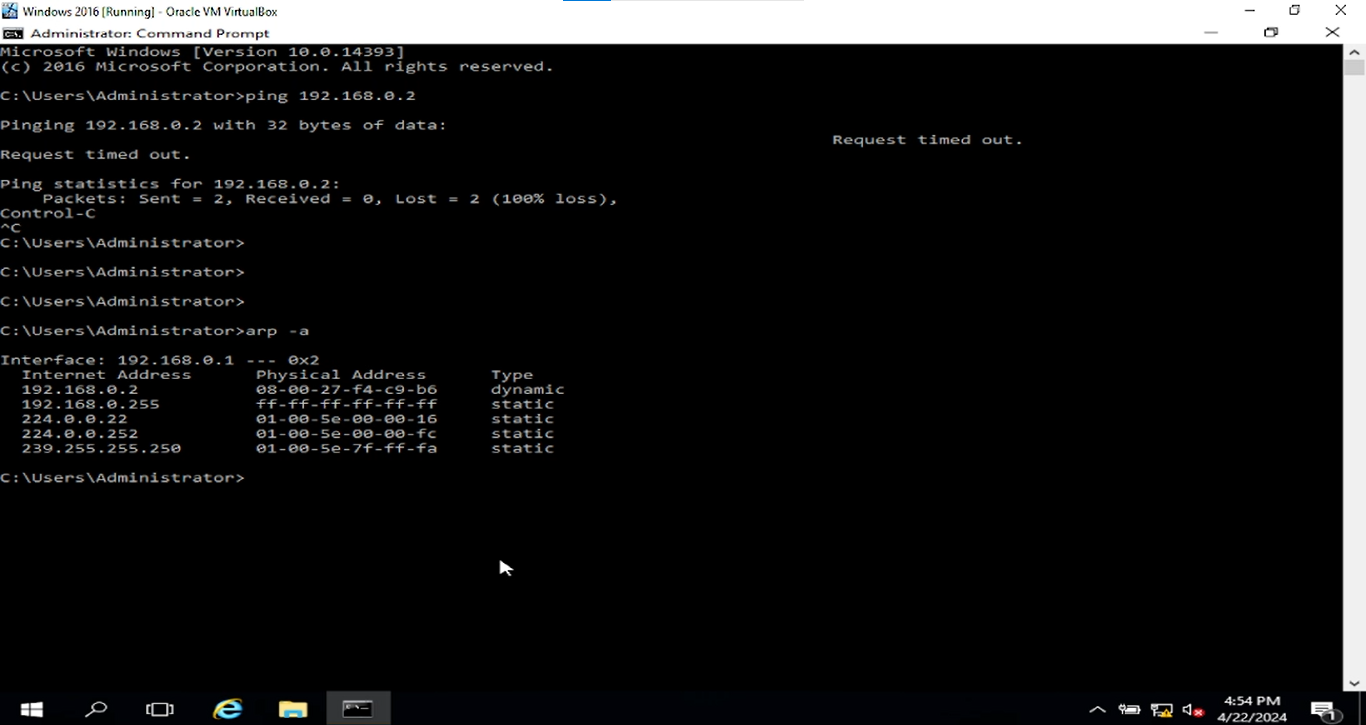
\includegraphics[width=0.9\linewidth]{figure//chapter5//lab5_3/ping_from_windows_server.png}
    \caption{Kết quả khi ping và arp -a}
    \label{fig:enter-label}
\end{figure}

Khi kiểm tra trên cả hai máy, ta thấy địa chỉ trùng khớp.

\noindent {\bf{Bước 4:}} Chuyển sang Kali Linux, vào Terminal. Truy cập vào \textbf{wireshark} và cấu hình cho chạy như ở phần 2. =

\noindent {\bf{Bước 5:}} Ở Windows Server, ta thực hiện ping lại như ở bước 3. Tại đây, bạn sẽ không thấy được dấu hiệu giao tiếp giữa hai máy Windows Server và Windows 10.

\begin{figure}[!htb]
    \centering
    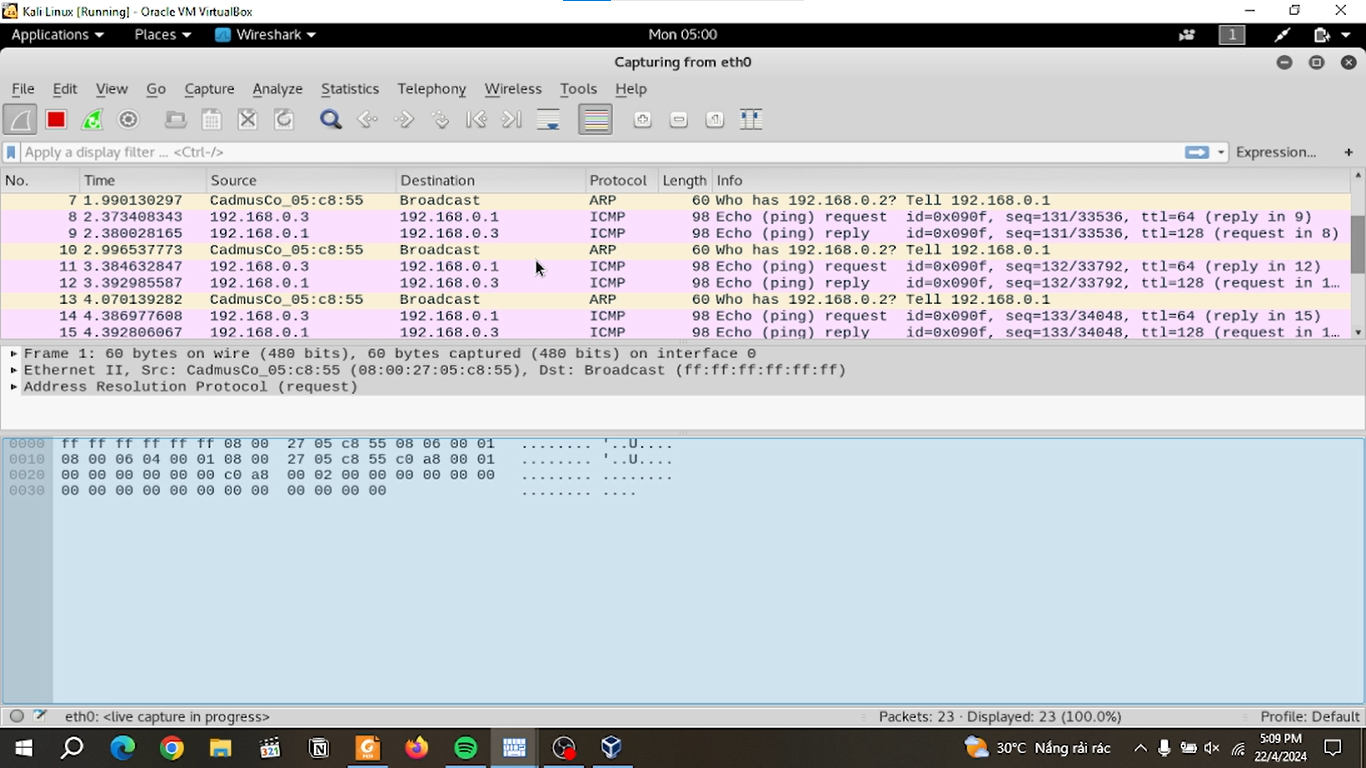
\includegraphics[width=0.9\linewidth]{figure//chapter5//lab5_3/first_test_ping.png}
    \caption{Kết quả capture khi ping từ Windows Server}
    \label{fig:enter-label}
\end{figure}

\newpage

\noindent {\bf{Bước 6:}} Vào \textbf{Application}, chọn \textbf{Sniffing/Spoofing}, chọn \textbf{ettercap-graphical}. 

\begin{figure}[!htb]
    \centering
    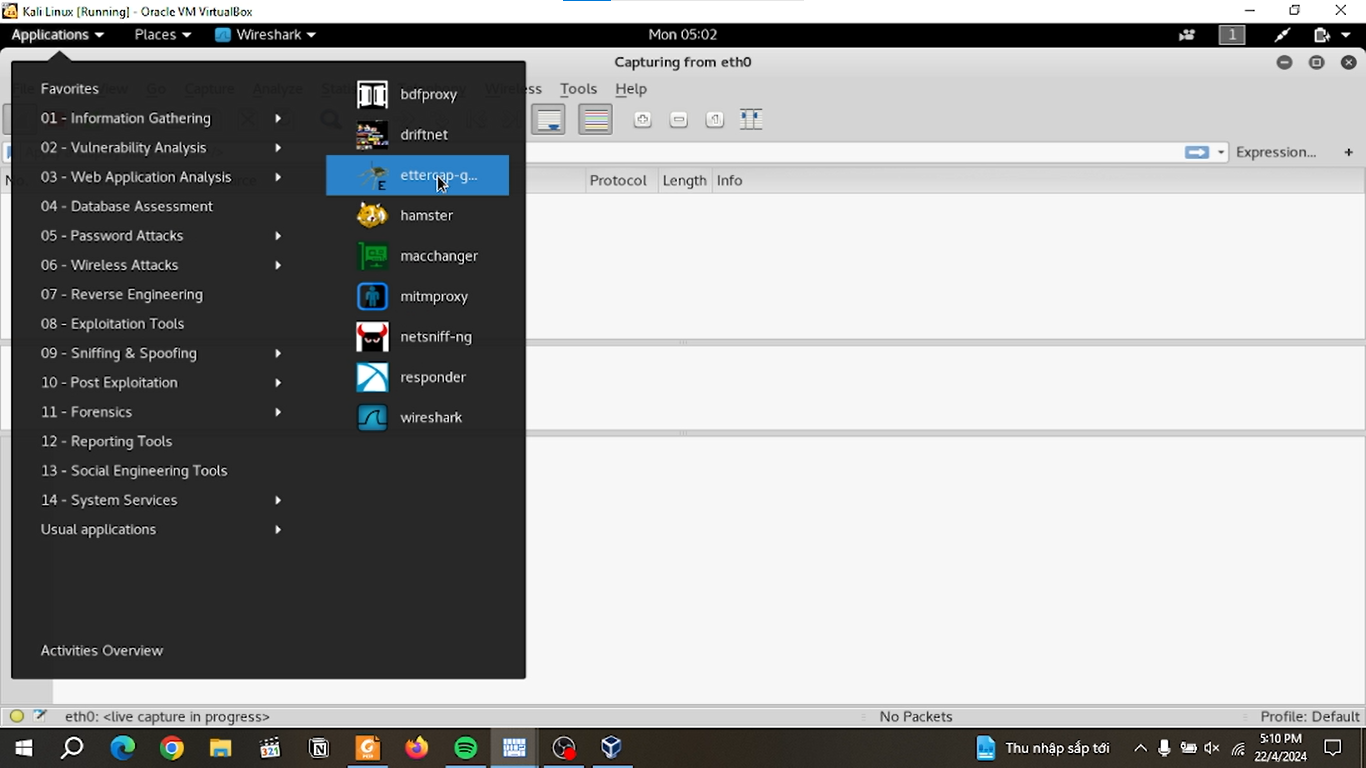
\includegraphics[width=1\linewidth]{figure//chapter5//lab5_3/ettercap_graphical.png}
    \caption{Chọn Ettercap-graphical}
    \label{fig:enter-label}
\end{figure}

Sau đó, từ Sniff, chọn \textbf{Unified sniffing}.

\begin{figure}[!htb]
    \centering
    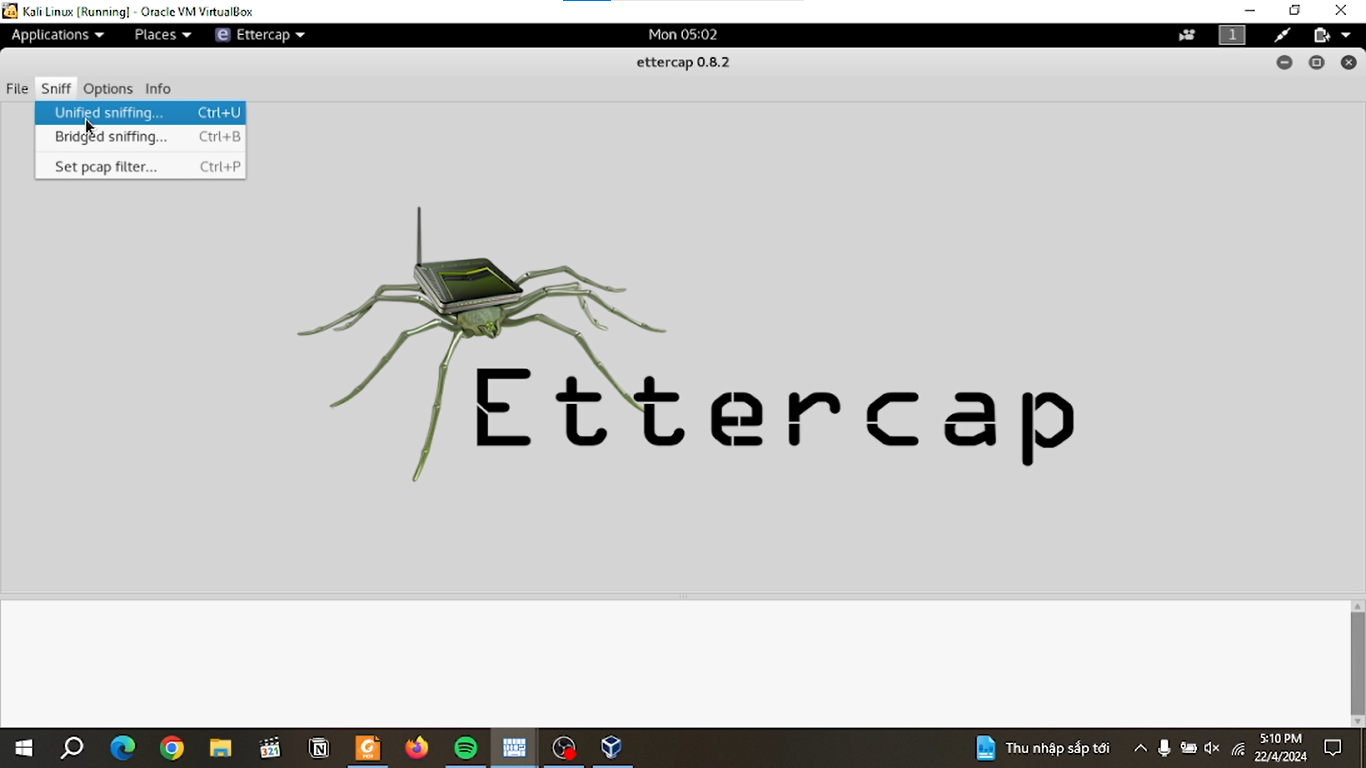
\includegraphics[width=1\linewidth]{figure//chapter5//lab5_3/sniffing.png}
    \caption{Chọn Unified Sniffing}
    \label{fig:enter-label}
\end{figure}

\newpage

\noindent {\bf{Bước 7:}} Ở \textbf{Hosts}, chọn \textbf{Scan for hosts}. Sau đó, từ \textbf{Hosts}, chọn \textbf{Hosts list}. Ở đây sẽ hiện ra địa chỉ IP và địa chỉ MAC của 2 máy ảo Windows.


\begin{figure}[!htb]
    \centering
    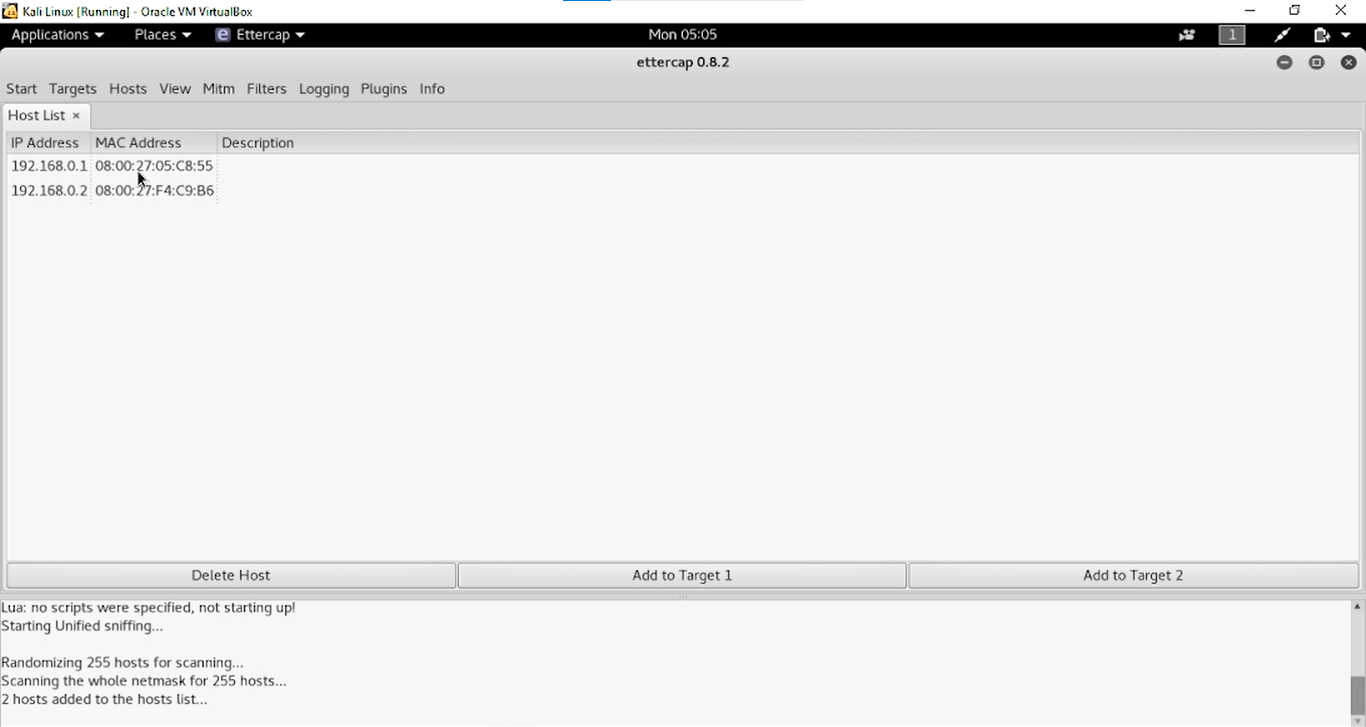
\includegraphics[width=1\linewidth]{figure//chapter5//lab5_3/host-list_2.png}
    \caption{Host Lists}
    \label{fig:enter-label}
\end{figure}


\noindent {\bf{Bước 8:}} Lần lượt chọn địa chỉ 2 máy, rồi chọn \textbf{Add to Target 1} và \textbf{Add to Target 2}. Sau đó chọn \textbf{Start sniffing}.

\begin{figure}[!htb]
    \centering
    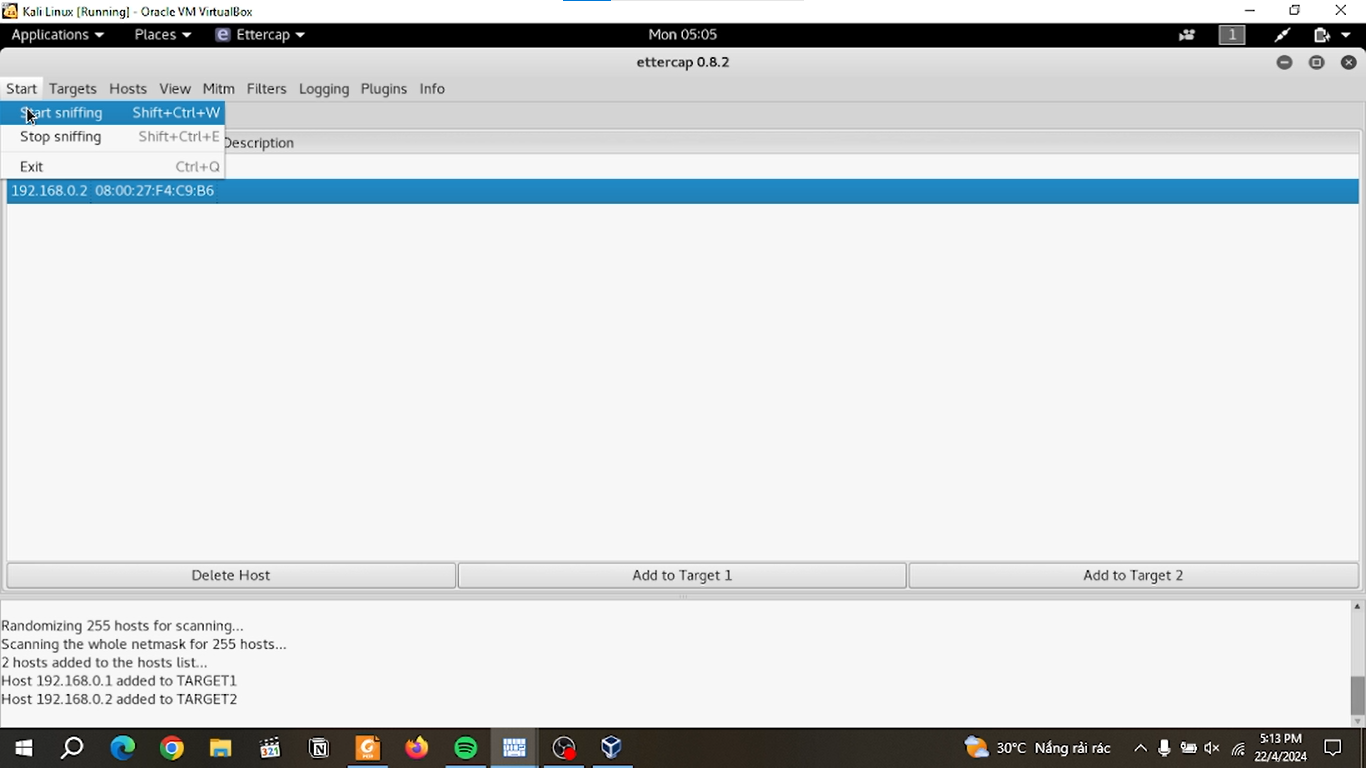
\includegraphics[width=1\linewidth]{figure//chapter5//lab5_3/start_sniffing.png}
    \caption{Bắt đầu sniffing}
    \label{fig:enter-label}
\end{figure}

\newpage

\noindent {\bf{Bước 9:}} Sau đó, ở menu \textbf{Mitm}, chọn \textbf{ARP Poisoning}. Sau đó, chọn \textbf{Sniff remote connections}.

\begin{figure}[!htb]
    \centering
    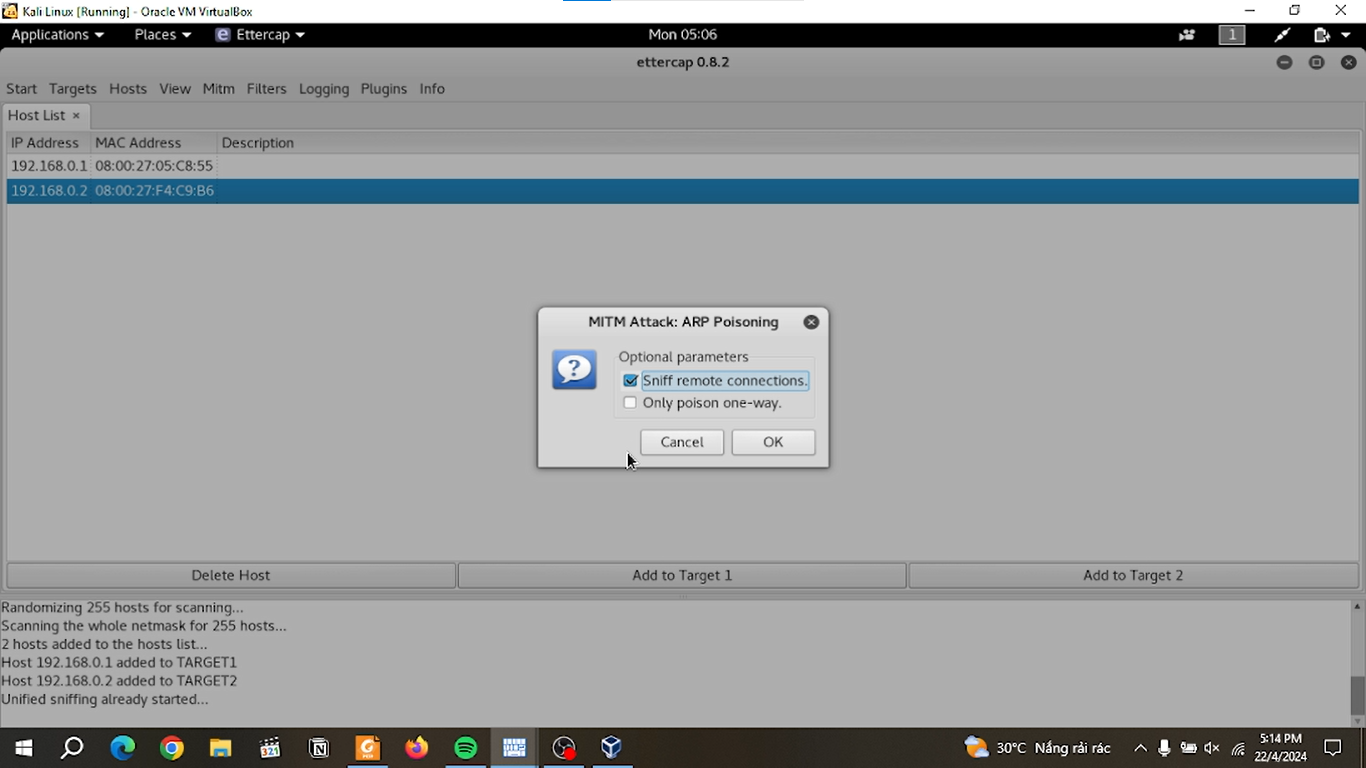
\includegraphics[width=1\linewidth]{figure//chapter5//lab5_3/arp-poisoning.png}
    \caption{Cài đặt ARP Poisoning}
    \label{fig:enter-label}
\end{figure}

\noindent {\bf{Bước 10:}} Từ Windows Server, ping tới Windows 10. Sau đó thực hiện \textbf{arp -a} thì kết quả cho thấy địa chỉ IP và địa chỉ MAC đều chuyển thành giống với của Kali Linux. 

\begin{figure}[!htb]
    \centering
    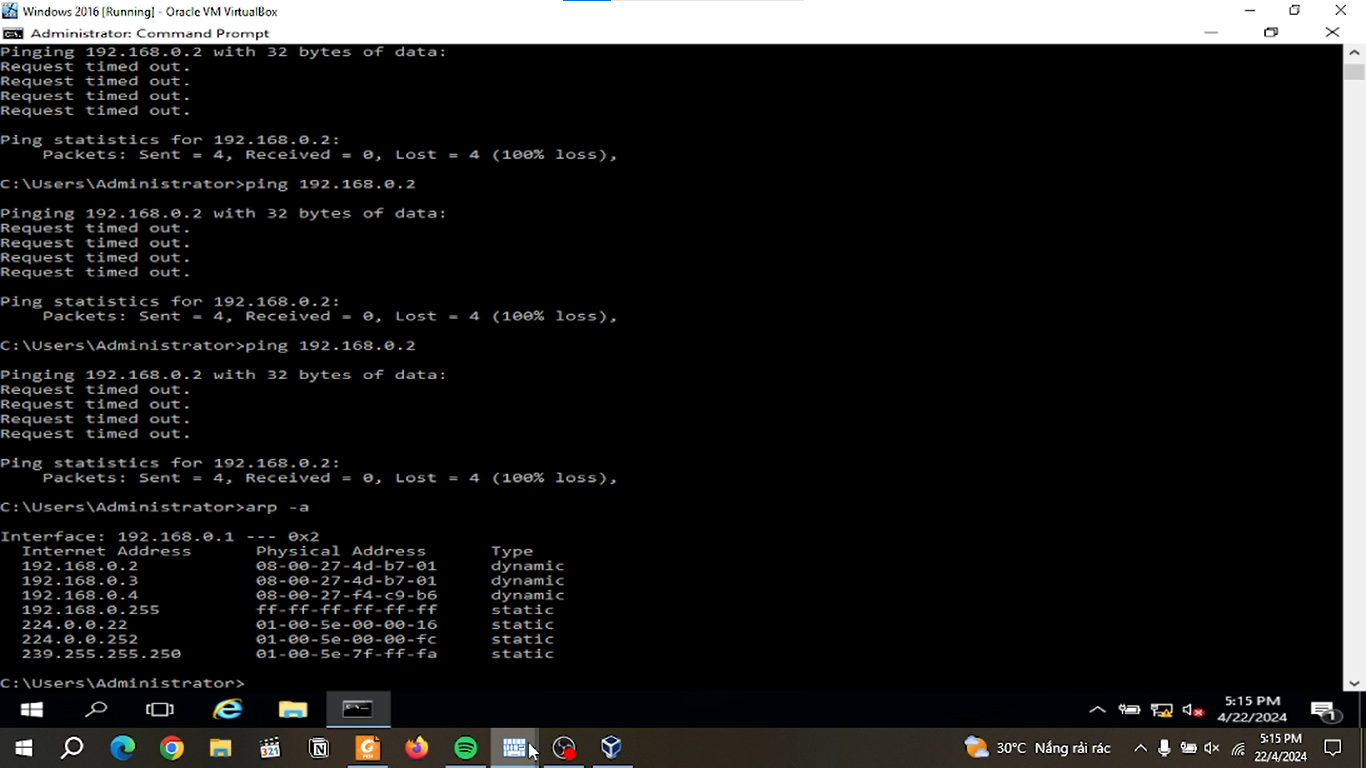
\includegraphics[width=1\linewidth]{figure//chapter5//lab5_3/result_arp.png}
    \caption{Kết quả sau khi ping và kiểm tra arp}
    \label{fig:enter-label}
\end{figure}

\newpage

\noindent {\bf{Bước 11:}} Thực hiện lại quá trình ping. Sau đó kiểm tra kết quả ở Wireshark. Lúc này đã có sự tương tác giữa hai máy Windows.

\begin{figure}[!htb]
    \centering
    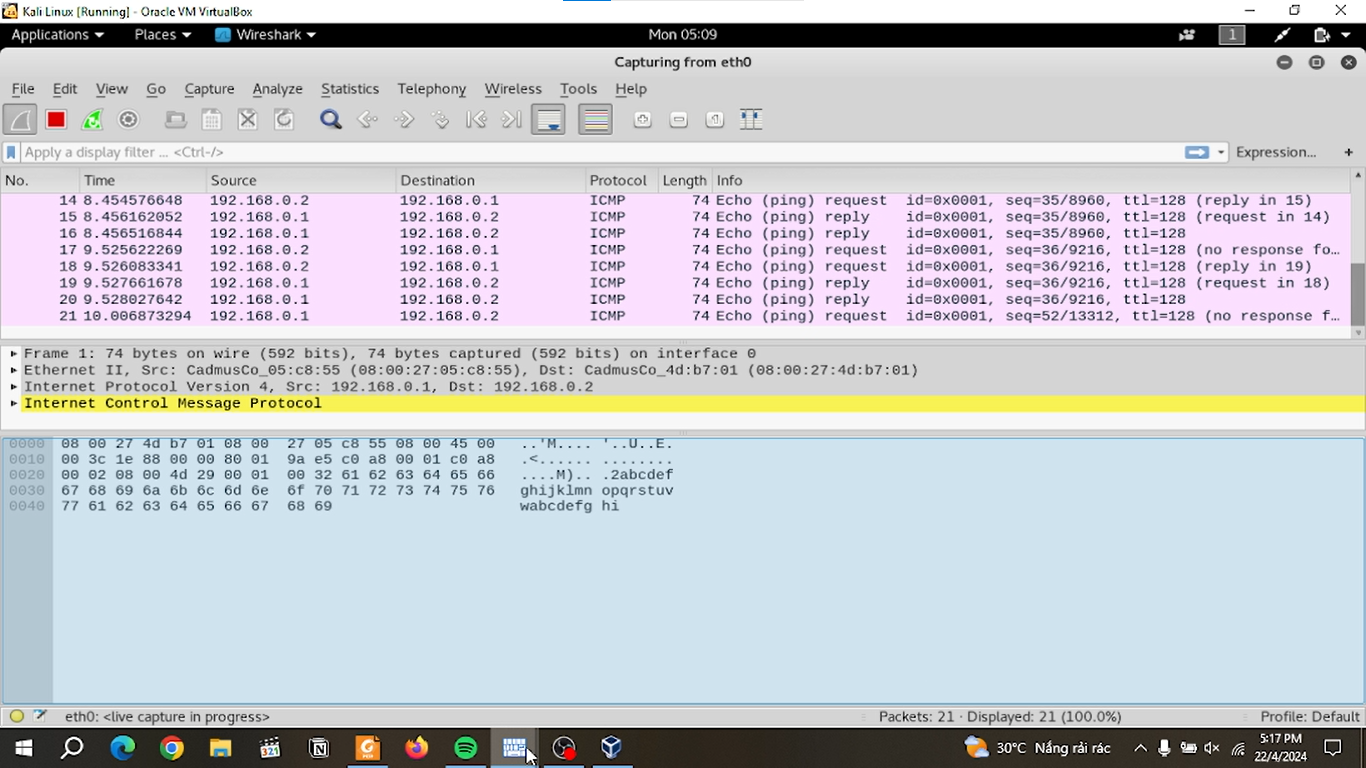
\includegraphics[width=1\linewidth]{figure//chapter5//lab5_3/final_result.png}
    \caption{Kết quả ở wireshark sau khi ping}
    \label{fig:enter-label}
\end{figure}

\subsection{Review Questions}

\noindent Câu 1:

A: ICMP redirection.

B: Buffer overflow.

C: Port stealing.

D: DHCP spoofing.

\noindent Câu 2: By altering the MAC addresses to those Kali Linux, the session was hijacked, and the pings were intercepted.

\noindent Câu 3: Because at this time, both Windows Server and Windows 10 were spoofed by Kali Linux, and interaction between them appeared in wireshark.

\noindent Câu 4: False

\noindent Câu 5:

A: /bin/cfg/etter.c.

\newpage

